\documentclass[12pt]{article}

\usepackage{amsmath, color}
\usepackage{mdwmath}
\usepackage{amssymb, epsf, epsfig, textcomp}
\renewcommand{\baselinestretch}{1.3}
\usepackage{a4wide}
\newcommand{\argmin}{\mathop{\mathrm{argmin}}}
\usepackage{caption}
\usepackage{subcaption}
\usepackage{mathtools}
\usepackage{listings}
\lstdefinestyle{myCustomMatlabStyle}{
	basicstyle=\ttfamily\footnotesize,
	breaklines=true,
	language=Matlab,
	numbers=left,
	stepnumber=1,
	numbersep=10pt,
	tabsize=4,
	showspaces=false,
	showstringspaces=false
}
\begin{document}
\noindent\rule{\textwidth}{2pt}
\begin{center}
{\bf Technical University of Crete}\\
{\bf School of Electrical and Computer Engineering} \\
Course: {\bf Convex Optimization} \\
Exercise 1 (100/1000) \\
Report Delivery Date: 2 November 2021 \\
Instructor: Athanasios P. Liavas \\
\end{center}
{\bf Student: }Alevrakis Dimitrios 2017030001\\
\rule{\textwidth}{.5pt}
\vskip .1cm
\noindent

\begin{enumerate}
\item 
Let $f:\mathbb{R}_{+} \rightarrow \mathbb{R}$, with $f(x) = \frac{1}{1+x}$. Let $x_0\in \mathbb{R}_{+}$,
and define the first- and second-order Taylor approximations of $f$ at $x_0$ as
\begin{equation}
\begin{split}
f_{(1)}(x) & = f(x_0) + f^{\prime}(x_0) (x-x_0), \cr
f_{(2)}(x) & = f(x_0) + f^{\prime}(x_0) (x-x_0) + \frac{1}{2} f^{\prime\prime}(x_0) (x-x_0)^2. \cr
\end{split} 
\end{equation}

\begin{enumerate}
\item 
Analytic expressions for functions $f^{\prime}$ and $f^{\prime\prime}$;
\begin{equation}
	\begin{split}
		f^{\prime}(x) &= -\frac{1}{(1+x)^2}, \cr
		f^{\prime\prime}(x) &= \frac{2}{(1+x)^3} \cr
	\end{split} 
\end{equation}

\item 
Plots of $f(x),f_{(1)}(x)$ and $f_{(2)}(x)$ for various $x_0$.
\begin{figure}
	\centering
	\begin{subfigure}[b]{\textwidth}
		\centering
		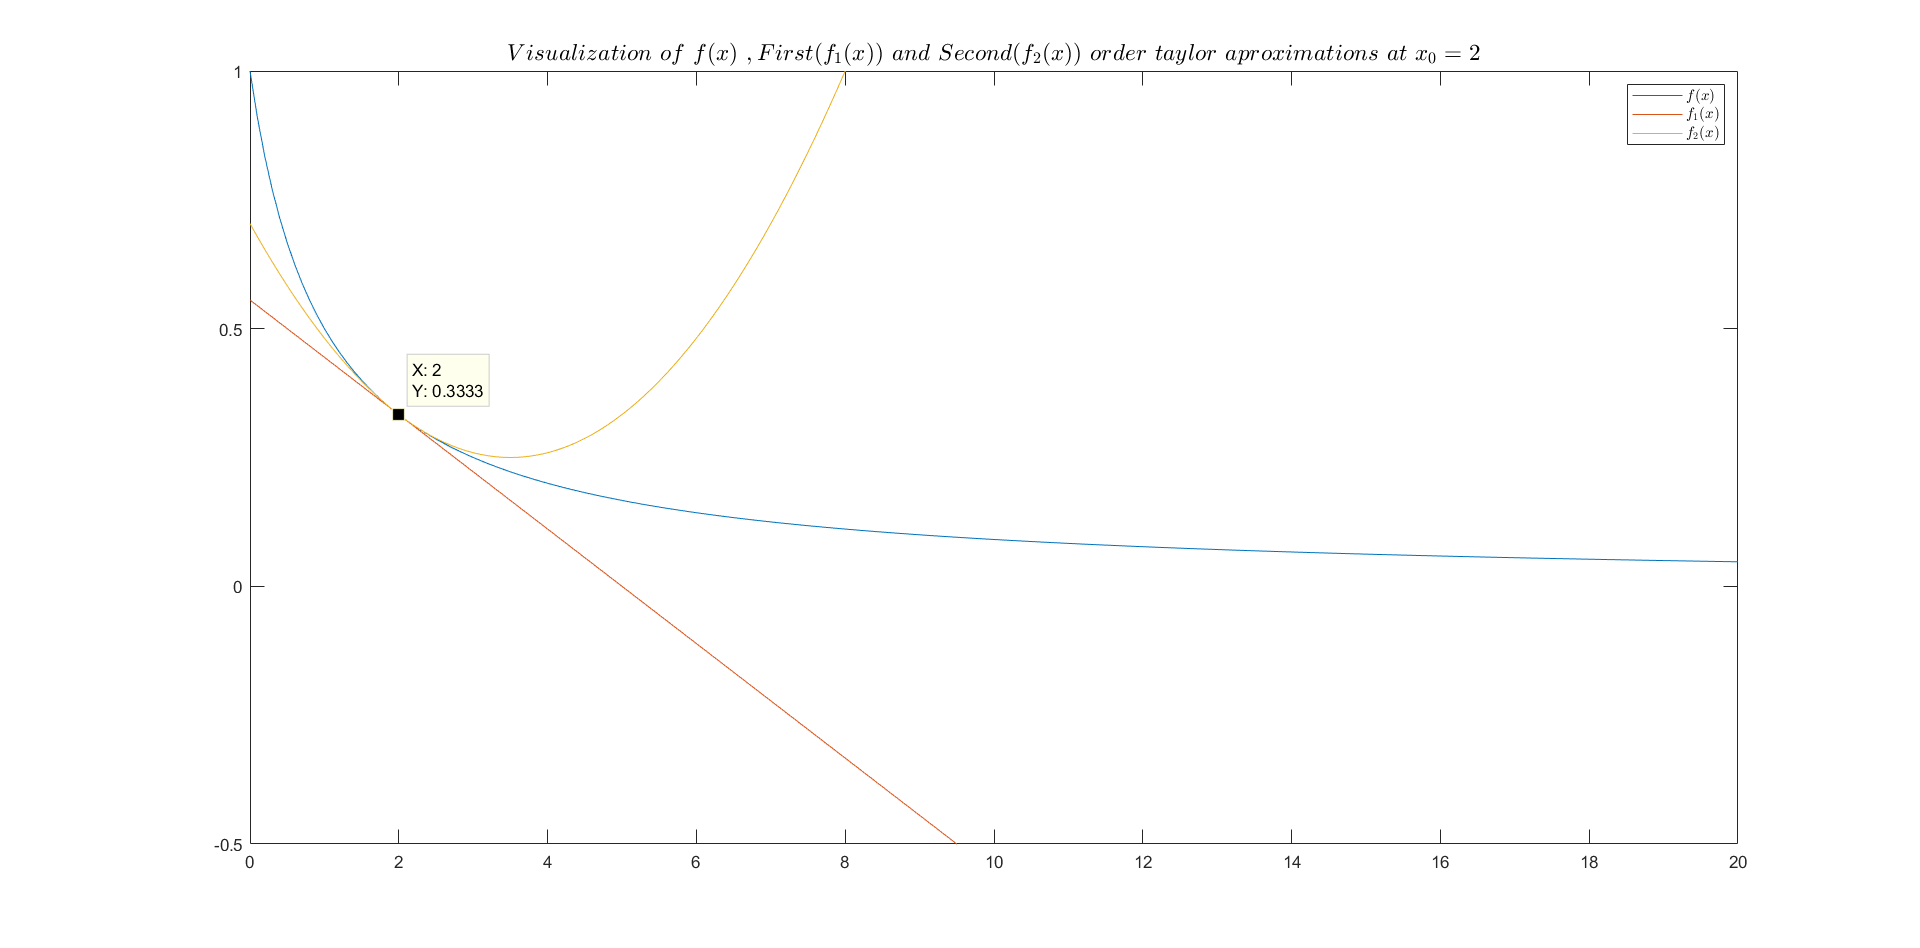
\includegraphics[width=\textwidth]{1.png}
		\caption{$x_0=2$}
		\label{fig:1}
	\end{subfigure}
	\begin{subfigure}[b]{\textwidth}
		\centering
		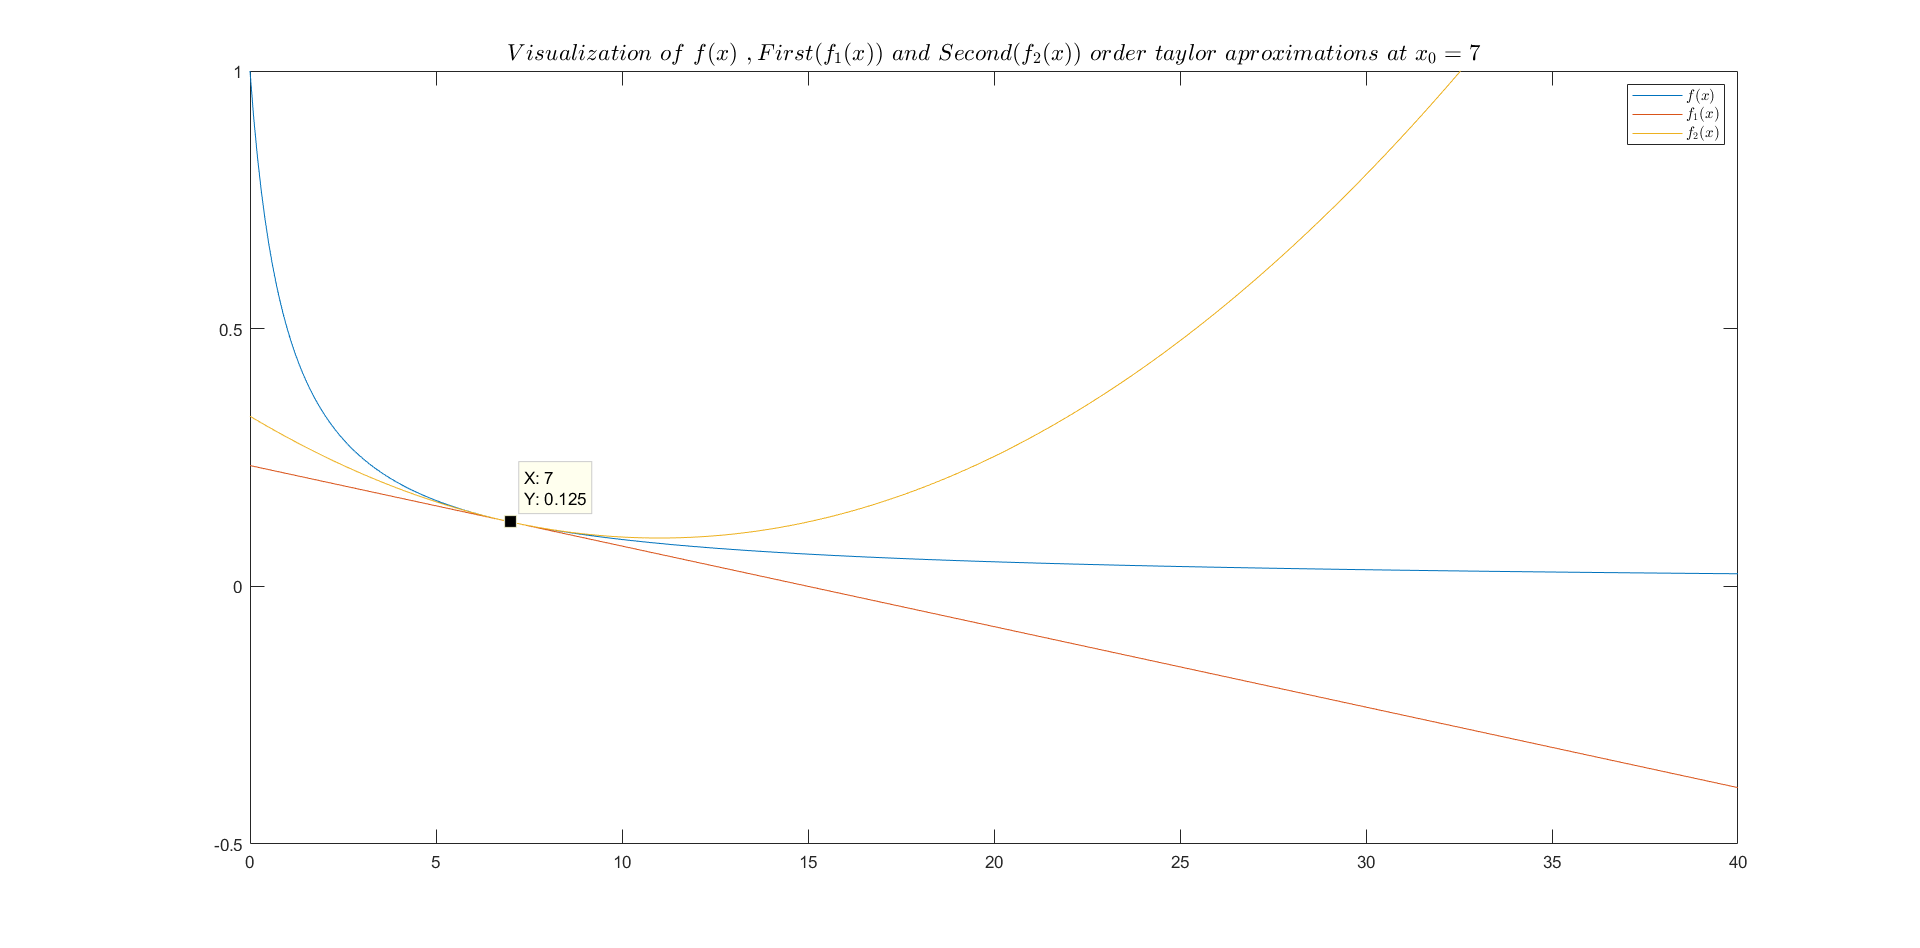
\includegraphics[width=\textwidth]{2.png}
		\caption{$x_0=7$}
		\label{fig:2}
	\end{subfigure}
\end{figure}
\begin{figure}
	\centering
	\begin{subfigure}[b]{\textwidth}
		\centering
		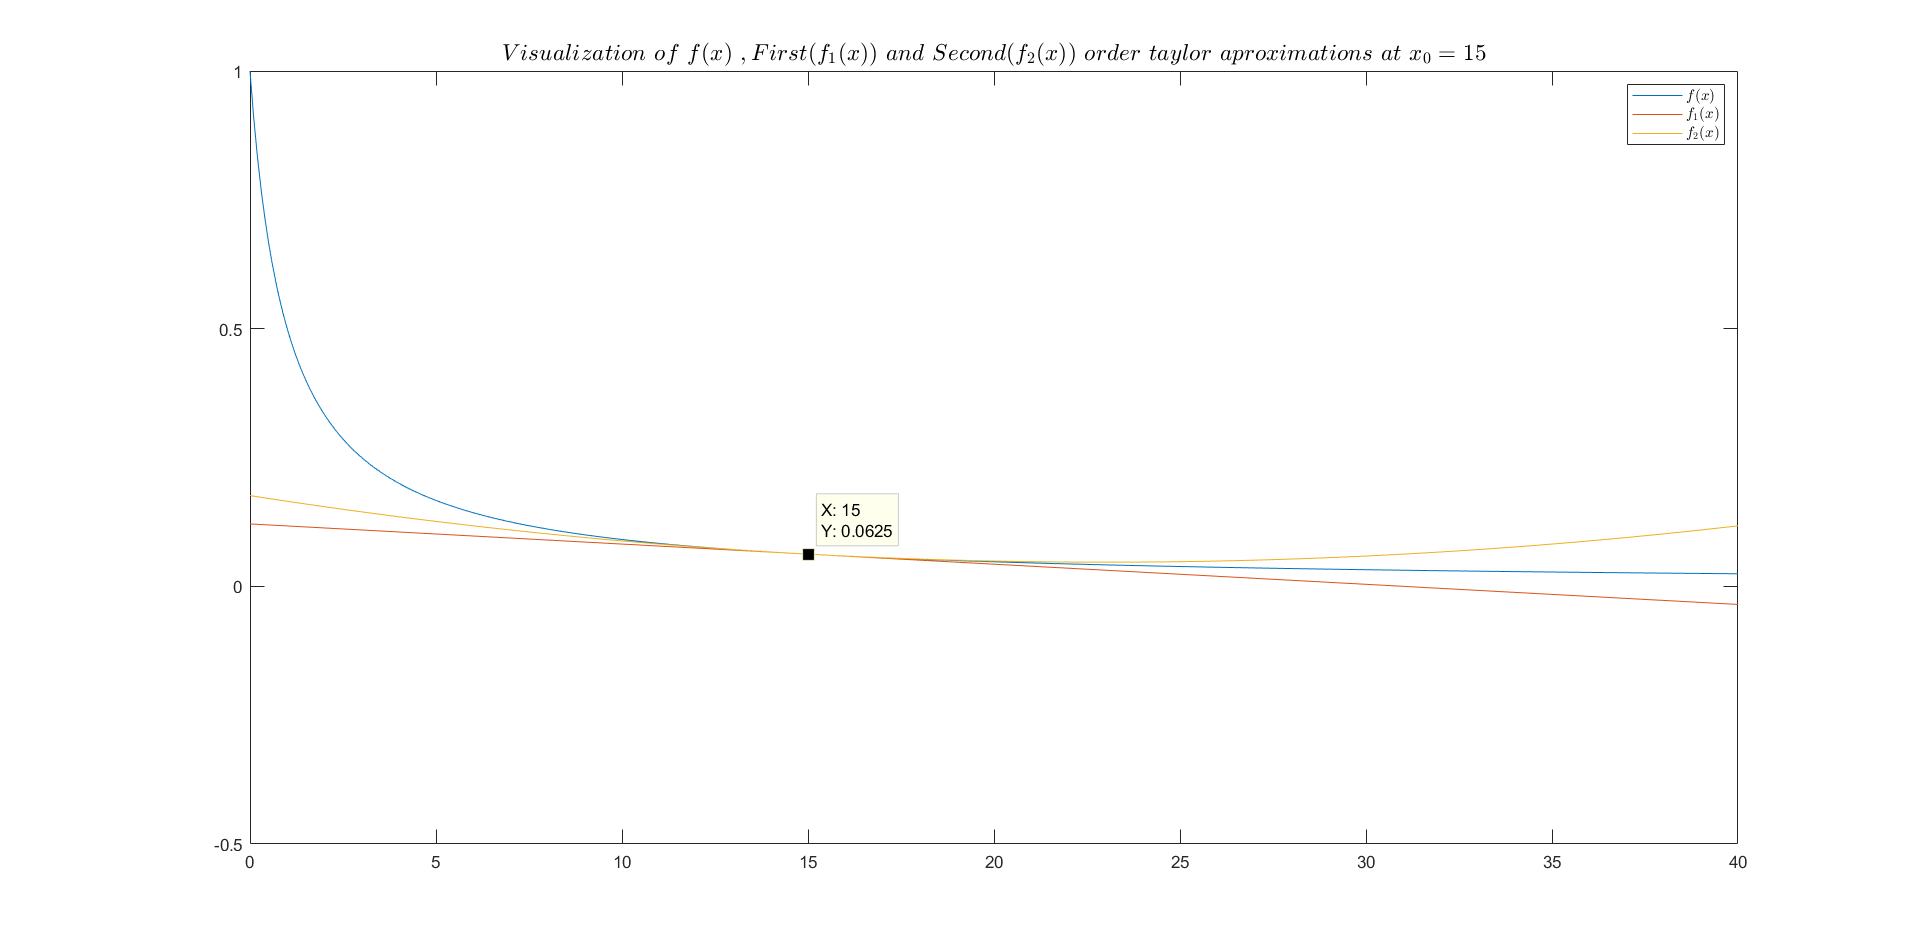
\includegraphics[width=\textwidth]{3.png}
		\caption{$x_0=15$}
		\label{fig:3}
	\end{subfigure}
	\begin{subfigure}[b]{\textwidth}
		\centering
		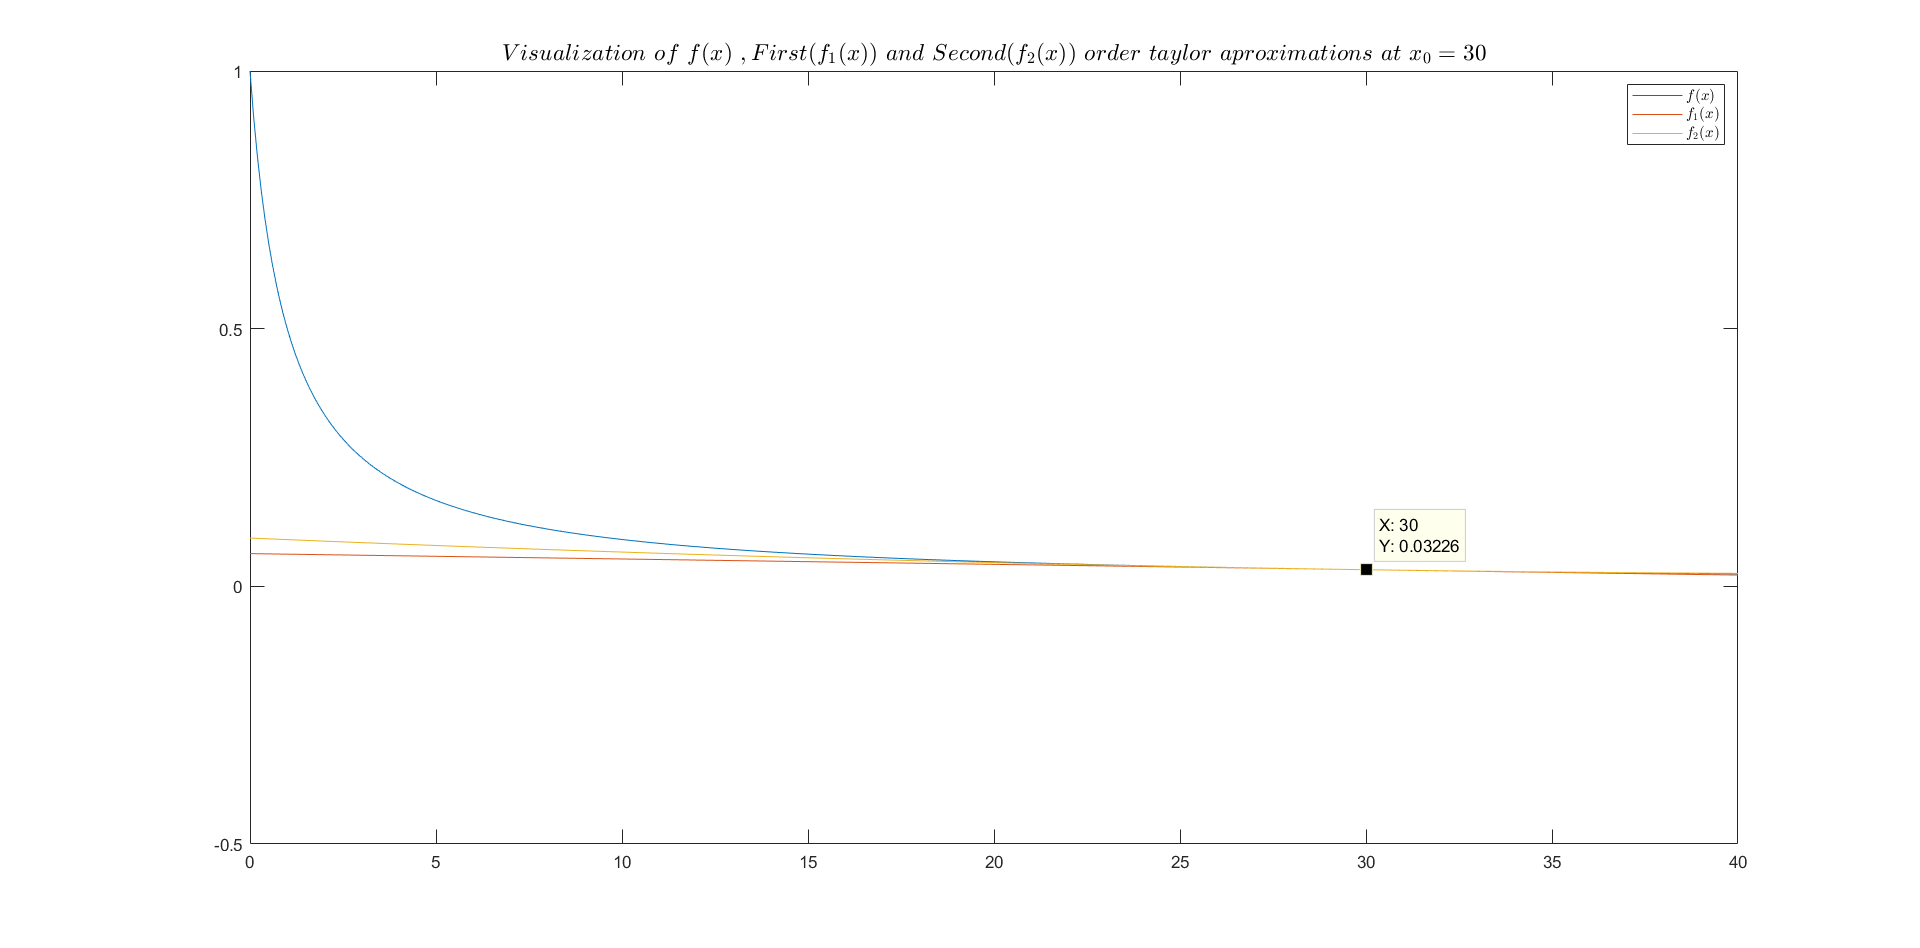
\includegraphics[width=\textwidth]{4.png}
		\caption{$x_0=30$}
		\label{fig:4}
	\end{subfigure}
\end{figure}
\end{enumerate}

As is confirmed from the above plots, since $f$ is convex, for every $x_0$,the first order taylor estimation is an underestimation of $f$ and the second derivative is always non-negative for every x.

\newpage
\item 
Let $f:\mathbb{R}_+^2 \rightarrow \mathbb{R}$, with $f(x_1,x_2) = \frac{1}{1+x_1+x_2}$.
\begin{enumerate}
\item Plotted f using mesh, for $x*=25$\\
\begin{figure}[h!]
	\centering
	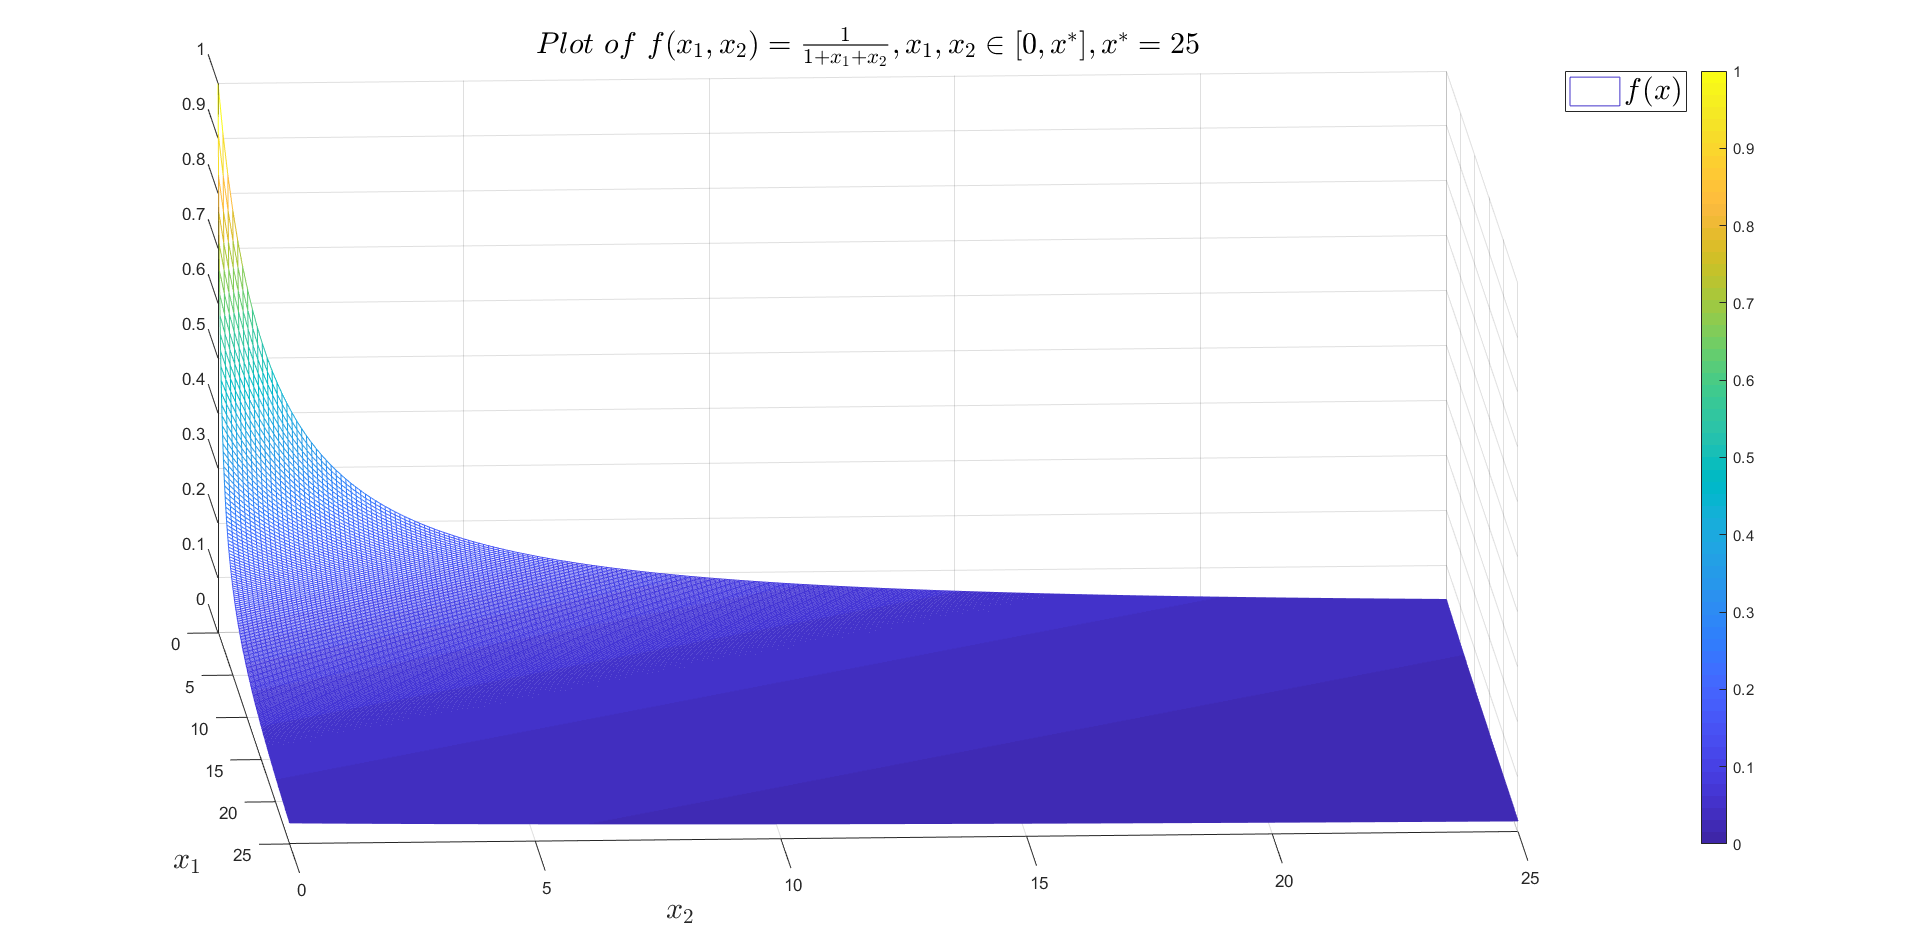
\includegraphics[width=0.8\textwidth]{5.png}
	\caption{$f(x_1,x_2)=\frac{1}{1+x_1+x_2},\ x_,1x_2\in [0,x^{*}],x^{*}=25$}
	\label{fig:5}
\end{figure}

\item
Level Sets of f:\\
\begin{figure}[h!]
	\centering
	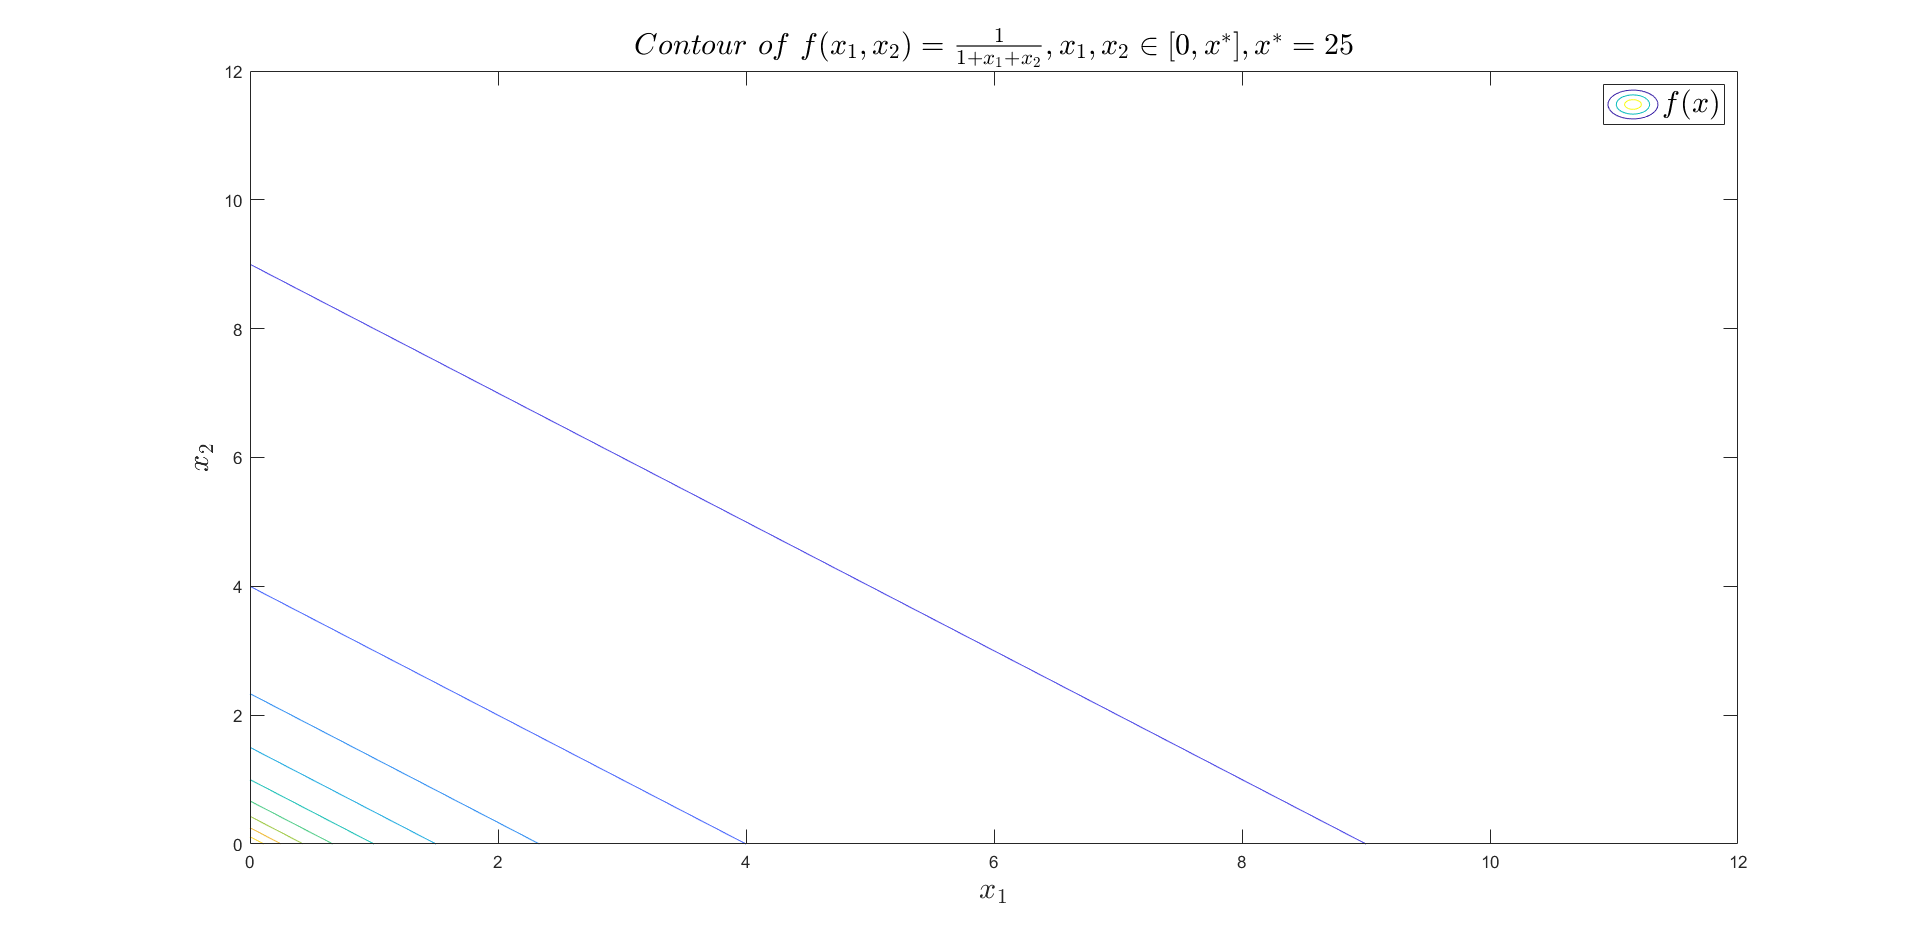
\includegraphics[width=0.8\textwidth]{6.png}
	\caption{Level Sets of f using contour}
	\label{fig:6}
\end{figure}\\
We observe that the level sets of f:\\
$S_c=\{x_1,x_2\in [0,x^{*}]:x_1+x_2=k | f(x_1,x_2)=c\}$. Since the level sets are described by a linear equation of $x_1$ and $x_2$, they are line segments parallel to each other.

\item 
First and Second Order Taylor approximations of $f$ at $x_0=(x_{01},x_{02})$:\\
Computation of the Gradient and the Hessian matrix;
\begin{equation}
	\begin{split}
		\nabla f(x) &=\begin{bmatrix}
			\frac{df}{dx_1} \\ \frac{df}{dx_2}
		\end{bmatrix} =
		\begin{bmatrix}
			-\frac{1}{(1+x_1+x_2)^2} \\ -\frac{1}{(1+x_1+x_2)^2} 
		\end{bmatrix}\\
		Hf(x) &=\begin{bmatrix}
			\frac{d^2}{d^2 x_1} & \frac{d^2}{dx_1dx_2}\\
			\frac{d^2}{dx_2dx_1} & \frac{d^2}{d^2 x_2}
		\end{bmatrix}=\begin{bmatrix}
			\frac{2}{(1+x_1+x_2)^3} & \frac{2}{(1+x_1+x_2)^3}\\
			\frac{2}{(1+x_1+x_2)^3} & \frac{2}{(1+x_1+x_2)^3}
		\end{bmatrix}
	\end{split}
\end{equation}
Computation of Taylor Approximations at $x_0=(x_{01},x_{02})$:
\begin{equation}
	\begin{split}
		f_1(x)&=f(x_0)+\nabla f(x_0)'(x-x_0)=f(x_0)+\begin{bmatrix}
			-\frac{1}{(1+x_{01}+x_{02})^2} \\ -\frac{1}{(1+x_{01}+x_{02})^2} 
		\end{bmatrix}'\begin{bmatrix}
		x_{1}-x_{01} \\ x_{2}-x_{02}
	\end{bmatrix}\\
	&=\frac{1}{1+x_{01}+x_{02}} -\frac{1}{(1+x_{01}+x_{02})^2}(x_1+x_2-x_{01}-x_{02})\\	
	f_2(x)&=f(x_0)+\nabla f(x_0)'(x-x_0) + \frac{1}{2}(x-x_0)'Hf(x)(x-x_0)\\
	&=f_1(x)+\frac{1}{2}\begin{bmatrix}
		x_{1}-x_{01} \\ x_{2}-x_{02}
	\end{bmatrix}'\begin{bmatrix}
		\frac{2}{(1+x_1+x_2)^3} & \frac{2}{(1+x_1+x_2)^3}\\
		\frac{2}{(1+x_1+x_2)^3} & \frac{2}{(1+x_1+x_2)^3}
	\end{bmatrix}\begin{bmatrix}
	x_{1}-x_{01} \\ x_{2}-x_{02}
\end{bmatrix}\\
	&=\frac{1}{1+x_{01}+x_{02}} -\frac{(x_1+x_2-x_{01}-x_{02})}{(1+x_{01}+x_{02})^2}+\frac{(x_1+x_2-x_{01}-x_{02})^2}{(1+x_1+x_2)^3}
	\end{split}
\end{equation}

\item 
Common plot $f$ and its first-order Taylor approximation at various $x_0=(x_{01},x_{02})$.
\begin{figure}[!h]
	\begin{subfigure}[b]{0.5\textwidth}
		\centering
		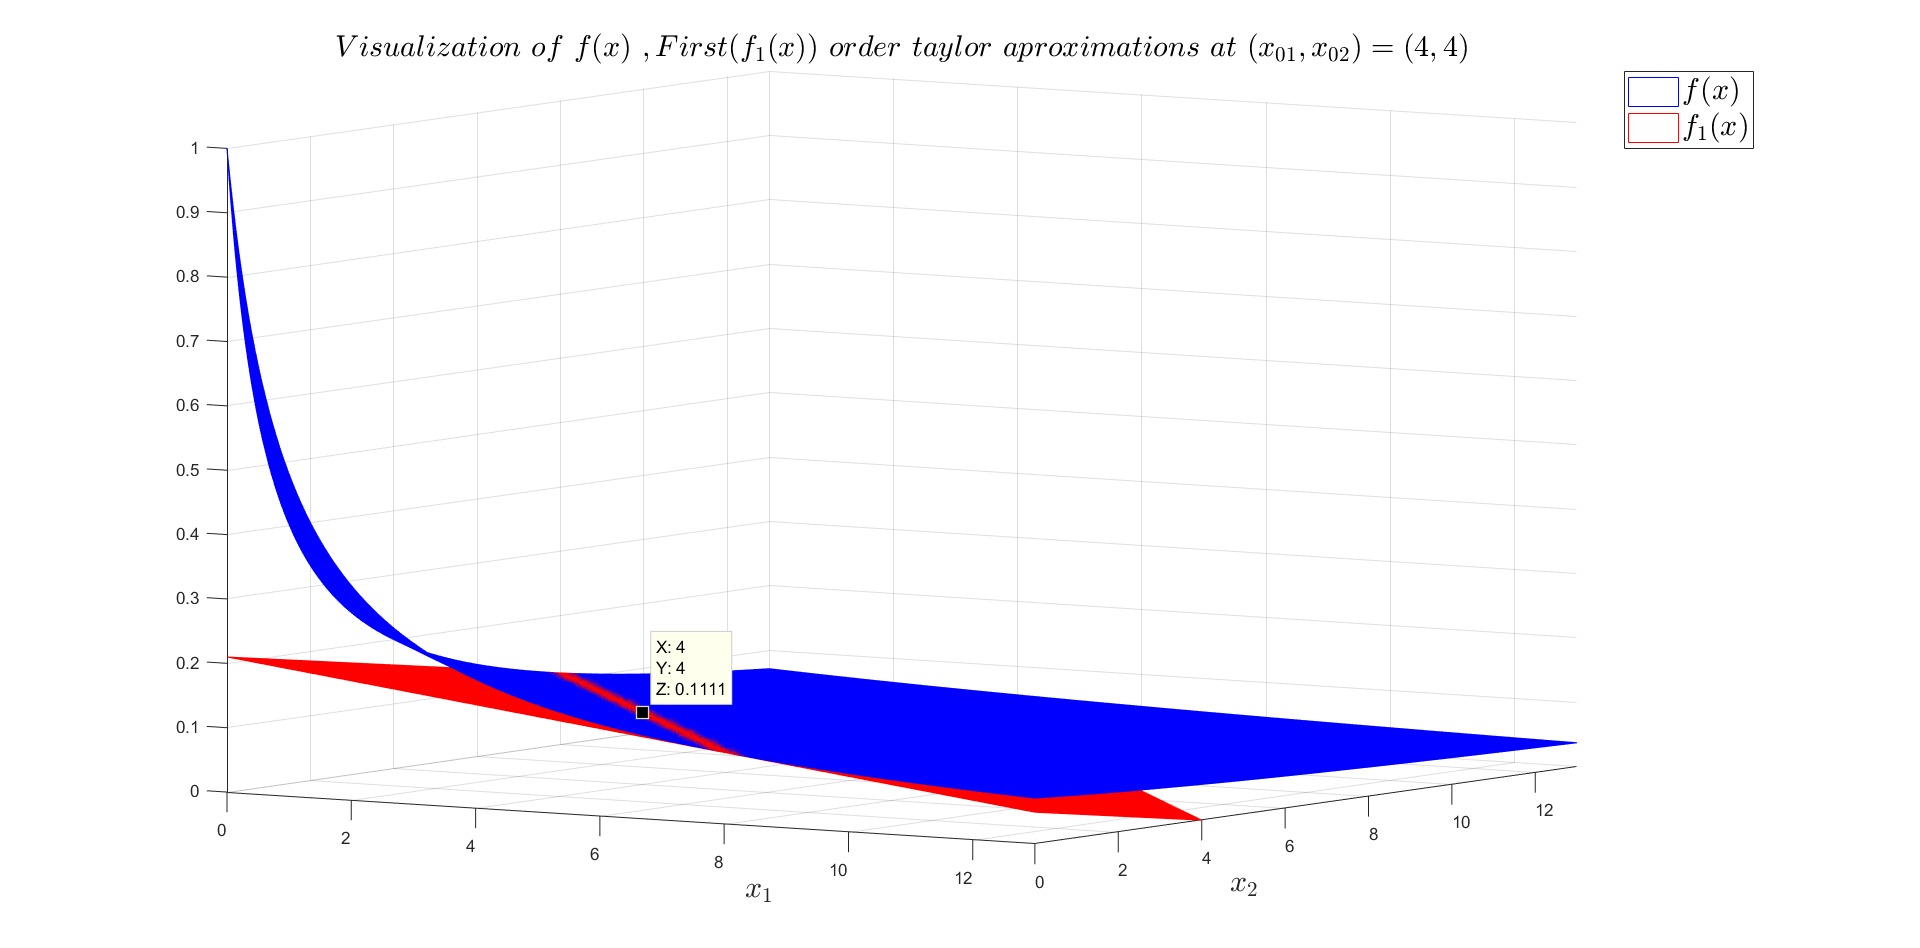
\includegraphics[width=\textwidth]{7a.png}
		\caption{$x_0=(4,4)$}
		\label{fig:7a}
	\end{subfigure}
	\hfill
	\begin{subfigure}[b]{0.5\textwidth}
		\centering
		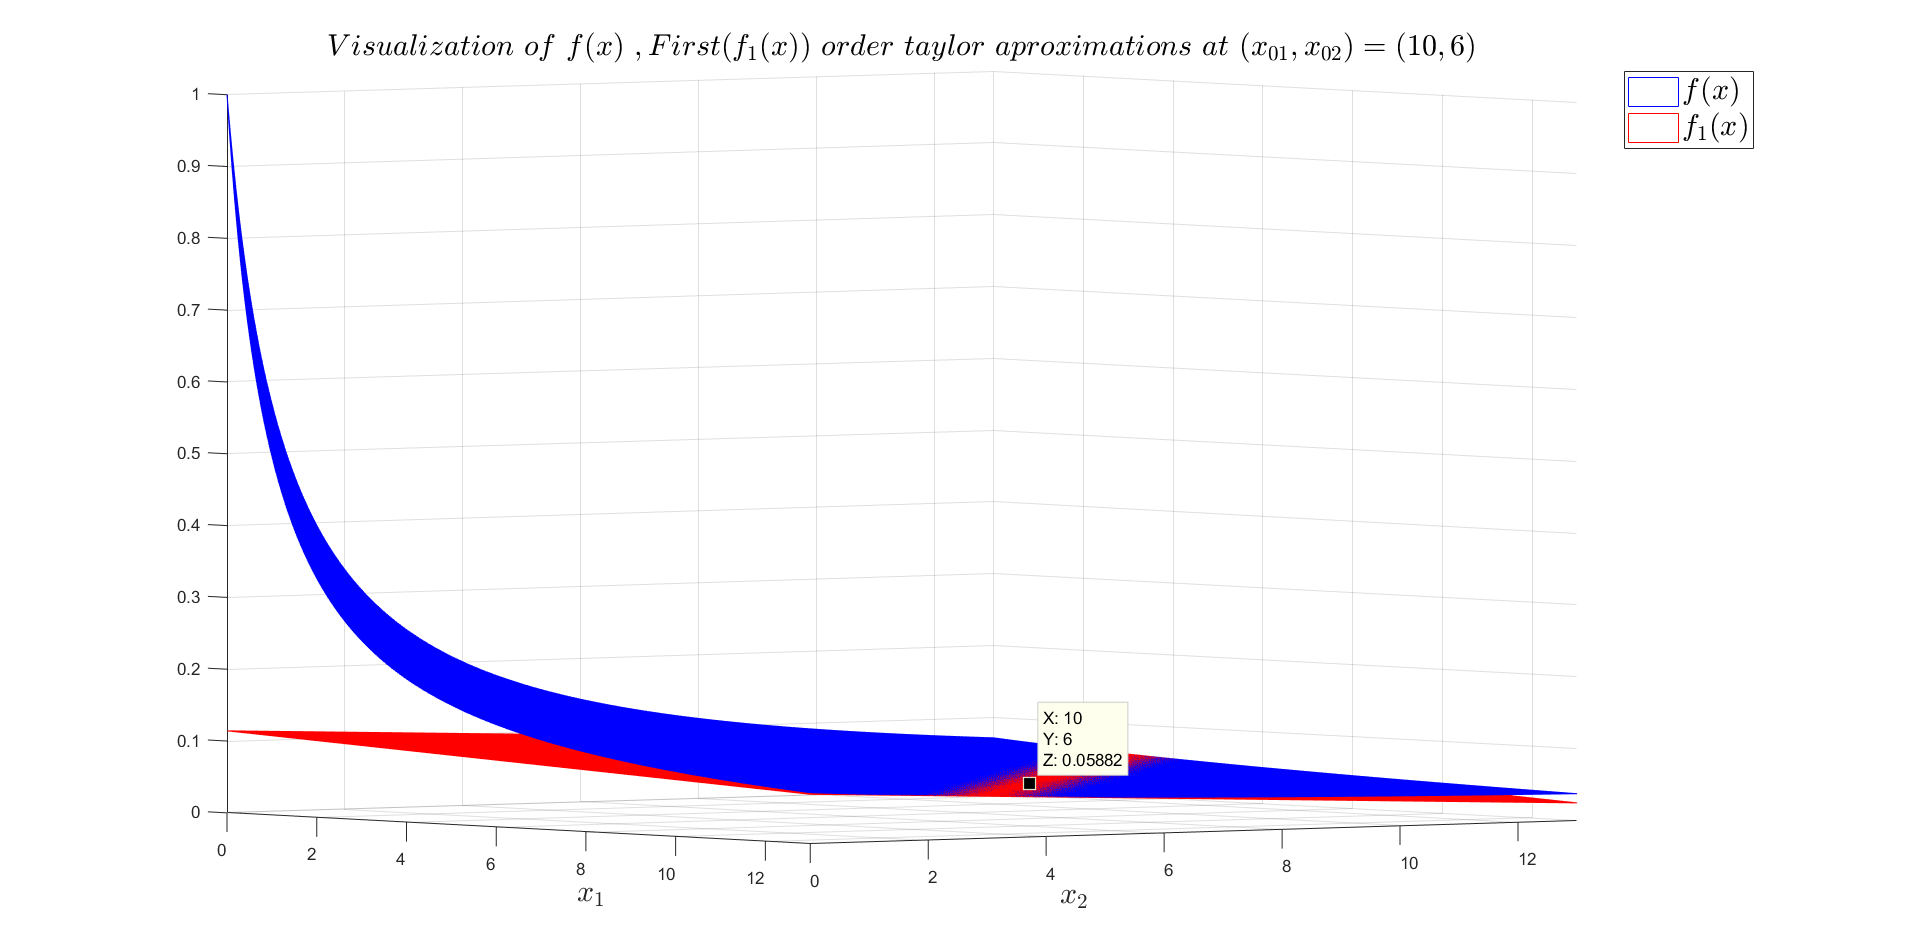
\includegraphics[width=\textwidth]{7b.png}
		\caption{$x_0=(10,6)$}
		\label{fig:7b}
	\end{subfigure}
\end{figure}
We notice that $f_1(x)$ is an underestimation of $f$ for every $x\in domf$ thus $f$ is convex.
\newpage
\item 
Common plot $f$ and its second-order Taylor approximation at various $x_0=(x_{01},x_{02})$.
\begin{figure}[!h]
	\begin{subfigure}[b]{0.5\textwidth}
		\centering
		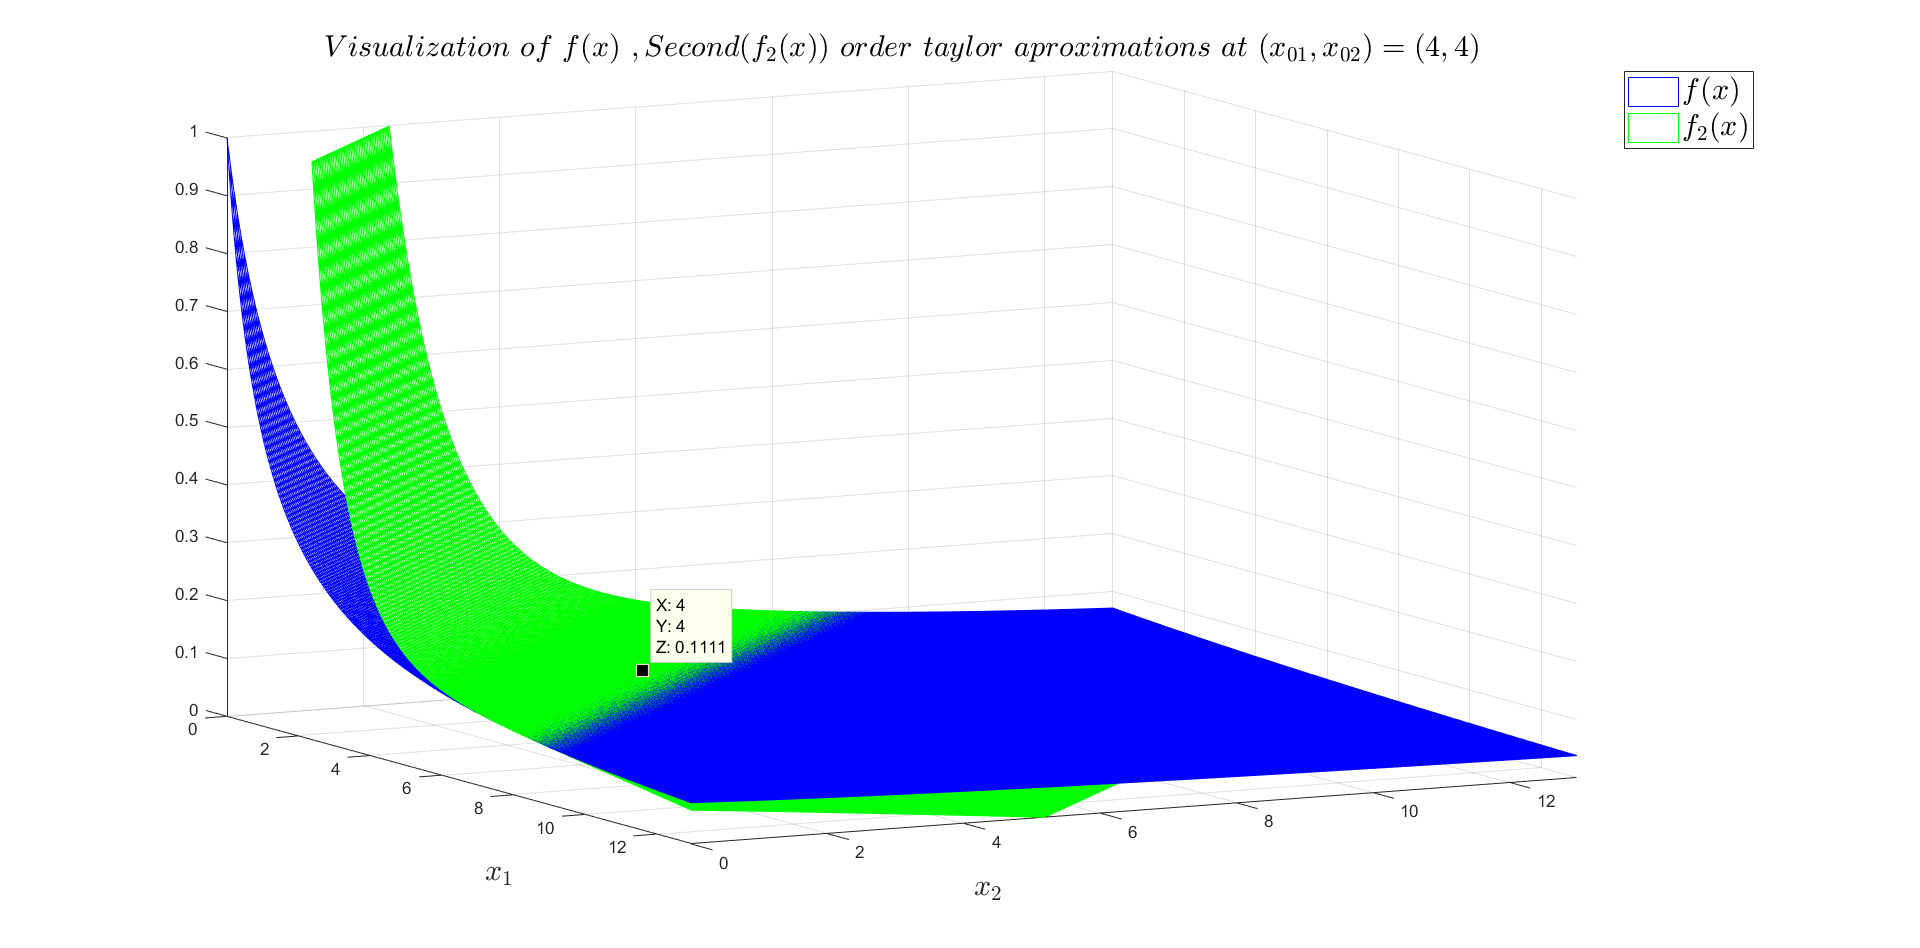
\includegraphics[width=\textwidth]{8a.png}
		\caption{$x_0=(4,4)$}
		\label{fig:8a}
	\end{subfigure}
	\hfill
	\begin{subfigure}[b]{0.5\textwidth}
		\centering
		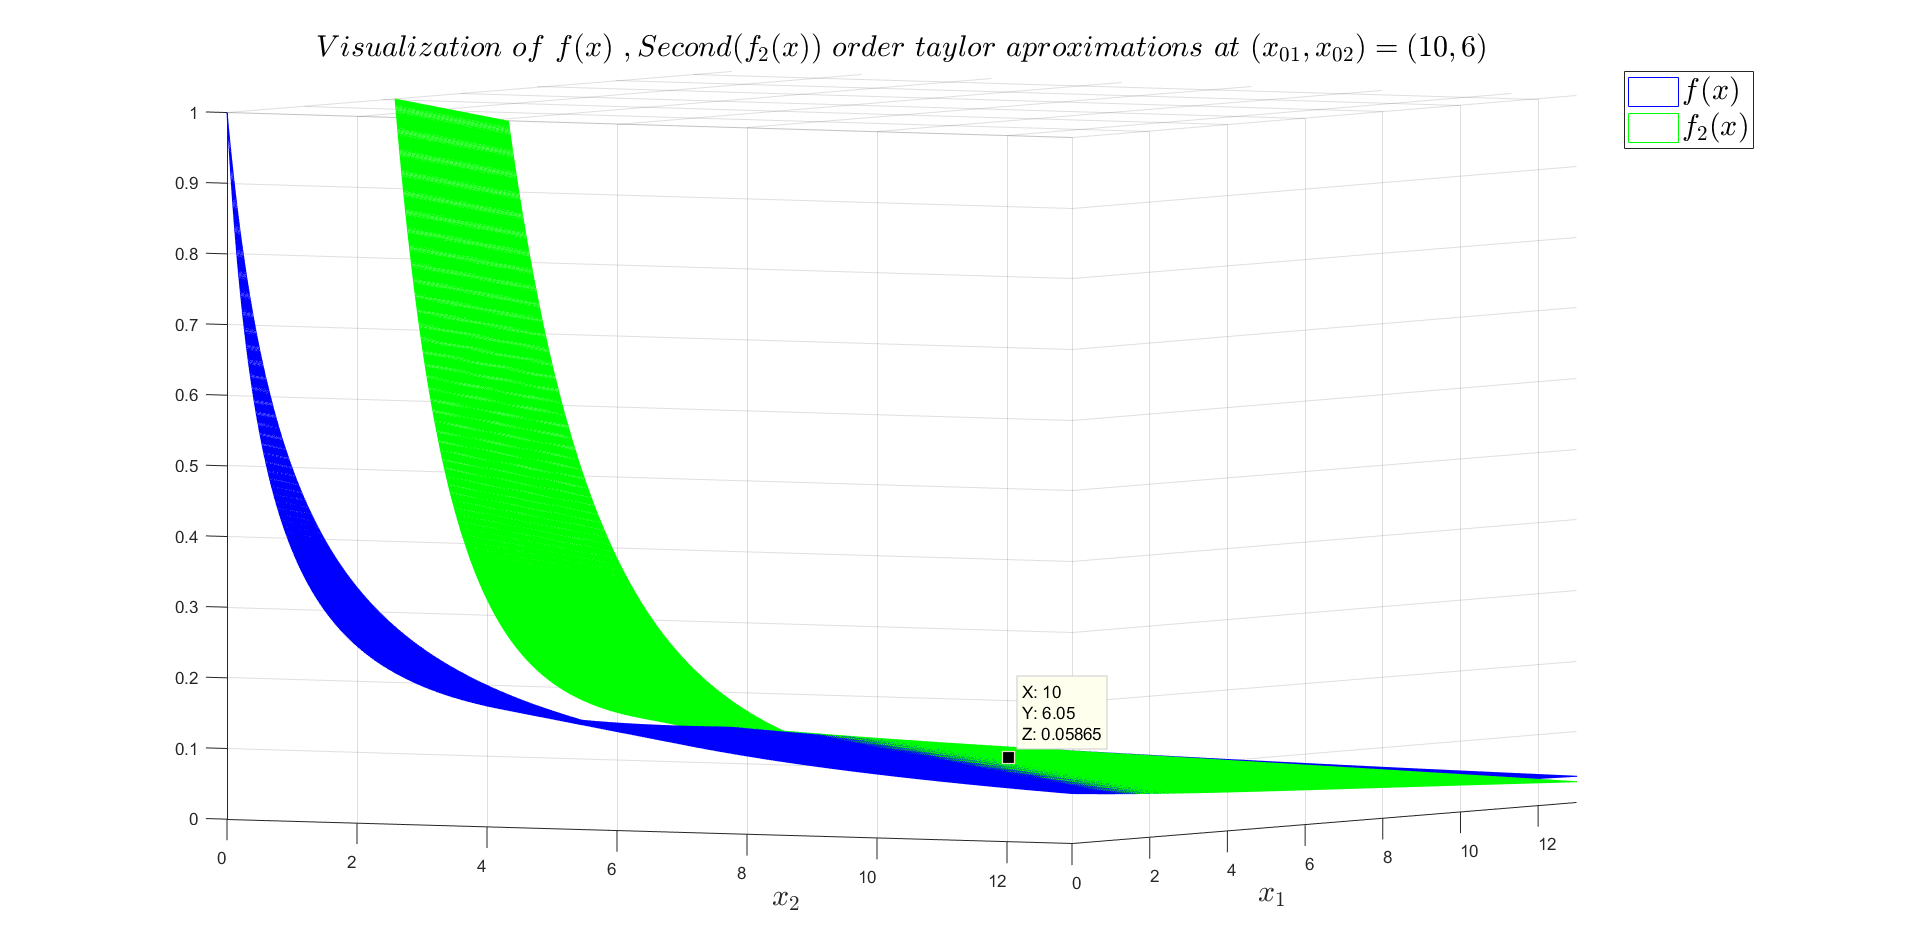
\includegraphics[width=\textwidth]{8b.png}
		\caption{$x_0=(10,6)$}
		\label{fig:8b}
	\end{subfigure}
\end{figure}

\end{enumerate}


\newpage 
\item
Let $\mathbb{S}_{{\bf a},b} = \{ {\bf x}\in\mathbb{R}^n \, | \, {\bf a}^T {\bf x} \le b \}$. 
\begin{enumerate}
\item 
Proof that $\mathbb{S}_{{\bf a}, b}$ is convex.\\
Let $x_1,x_2\in S_{{\bf a}, b}$ then for $0\leq\theta\leq1$:
\begin{equation}
	\begin{split}
		&\begin{rcases}
			{\bf a}^{T}{\bf x_1}\leq b \iff \theta	{\bf a}^{T}{\bf x_1}\leq \theta b \\
				{\bf a}^{T}{\bf x_2}\leq b \iff (1-\theta)	{\bf a}^{T}{\bf x_2}\leq (1-\theta) b
		\end{rcases}\iff \\
		&\theta	{\bf a}^{T}{\bf x_1}+(1-\theta)	{\bf a}^{T}{\bf x_2}\leq \theta b+(1-\theta) b\iff\\
		&{\bf a}^{T}(\theta{\bf x_1}+(1-\theta)	{\bf x_2})\leq b
	\end{split}
\end{equation}
Therefore the convex combination of any $x_1,x_2\in \mathbb{S}_{{\bf a},b}$ belongs in $\mathbb{S}_{{\bf a},b}$. Therefore $\mathbb{S}_{{\bf a},b}$ is convex.

\item 
In order to prove that $\mathbb{S}_{{\bf a},b}$ is not affine we need to show that there exists an affine combination of ${\bf x}\in  \mathbb{S}_{{\bf a},b}$ which is not in  $\mathbb{S}_{{\bf a},b}$.\\
Let ${\bf a}^T=[2,3]$ and $b=20$.\\
We choose:
\begin{equation}
	\begin{split}
		&{\bf x_1}^T=[2,4]\ :\ {\bf a}^T{\bf x_1}=16<b\\
		&{\bf x_2}^T=[6,2]\ :\ {\bf a}^T{\bf x_1}=18<b\\
		&{\bf x_3}^T=[1,3]\ :\ {\bf a}^T{\bf x_1}=11<b\\
	\end{split}
\end{equation}
And let $\theta_1=0.2$, $\theta_2=1.5$ $\theta_2=-0.7$, for which is true that $\theta_1+\theta_2+\theta_3=1$\\
So:$\theta_1{\bf a}^T{\bf x_1}+\theta_2{\bf a}^T{\bf x_2}+\theta_3{\bf a}^T{\bf x_3} = 0.2*16+1.5*18-0.7*11=22.5>b$\\
Therefore $\mathbb{S}_{{\bf a},b}$ is not affine.

\end{enumerate}


\item
Let ${\bf z\in \mathbb{R}^n}$ co-linear to ${\bf a}$. Then ${\bf z}=n{\bf a},n\in R*$.\\
In order for ${\bf z}$ to lie in $\mathbb{H}_{\bf a}$ it must satisfy the equality:\\
${\bf a}^T{\bf z}=b \iff n{\bf a}^T{\bf a}=b \iff n=\frac{b}{||{\bf a}||_2^2}$.\\
Therefore ${\bf z}=\frac{b}{||{\bf a}||_2^2}{\bf a}$

\item 
Check whether the following functions are convex or not.
\begin{enumerate}
\item
$f:\mathbb{R}_{+}\rightarrow \mathbb{R}$, with $f(x)=\frac{1}{1+x}$;\\
\begin{equation}
	\begin{split}
		f^{\prime}(x) &= -\frac{1}{(1+x)^2}, \cr
		f^{\prime\prime}(x) &= \frac{2}{(1+x)^3} \cr
	\end{split} 
\end{equation}
Since $f^{\prime\prime}(x)\succcurlyeq0 \forall x\in \mathbb{R}_{+}$, f convex.

\item 
$f:\mathbb{R}_+^2 \rightarrow \mathbb{R}$, with $f(x_1,x_2) = \frac{1}{1+x_1+x_2}$;
\begin{equation}
	\begin{split}
		\nabla f(x) &=\begin{bmatrix}
			\frac{df}{dx_1} \\ \frac{df}{dx_2}
		\end{bmatrix} =
		\begin{bmatrix}
			-\frac{1}{(1+x_1+x_2)^2} \\ -\frac{1}{(1+x_1+x_2)^2} 
		\end{bmatrix}\\
		Hf(x) &=\begin{bmatrix}
			\frac{d^2}{d^2 x_1} & \frac{d^2}{dx_1dx_2}\\
			\frac{d^2}{dx_2dx_1} & \frac{d^2}{d^2 x_2}
		\end{bmatrix}=\begin{bmatrix}
			\frac{2}{(1+x_1+x_2)^3} & \frac{2}{(1+x_1+x_2)^3}\\
			\frac{2}{(1+x_1+x_2)^3} & \frac{2}{(1+x_1+x_2)^3}
		\end{bmatrix}
	\end{split}
\end{equation}
In order for f to be convex, $Hf(x)$ must be positive definite $\Rightarrow\ {\bf z}^T{\bf H}f(x){\bf z}\ge 0\forall z\in\mathbb{R}^2-\{{\bf 0}\}$.\\
Let ${\bf z}=(a,b)^T \in \mathbb{R}^2$.\\
\begin{equation}
	\begin{split}
		{\bf z}^T{\bf H}f(x){\bf z}= &\\ &a^2\frac{2}{(1+x_1+x_2)^3}+ab\frac{2}{(1+x_1+x_2)^3}+ab\frac{2}{(1+x_1+x_2)^3}+b^2\frac{2}{(1+x_1+x_2)^3} \\
		&=2\frac{a^2+2ab+b^2}{(1+x_1+x_2)^3} = 2\frac{(a+b)^2}{(1+x_1+x_2)^3} \ge0 \forall {\bf z}\in\mathbb{R}^2,\ {\bf x}\in\mathbb{R}_{++}
	\end{split}
\end{equation}
Therefore $Hf(x)\succcurlyeq0 \forall x\in \mathbb{R}_{++}$ and f is  convex. 
\item 
$f:\mathbb{R}_{++} \rightarrow \mathbb{R}$, with $f(x)=x^a$.
\begin{equation}
	\begin{split}
		f^{\prime}(x) &=ax^{a-1}, \cr
		f^{\prime\prime}(x) &= a(a-1)x^{a-2} \cr
	\end{split} 
\end{equation}
\begin{enumerate}
\item if $a \leq 0 \iff a-1\leq-1\leq0 \implies a(a-1)\ge0$\\
 Since $f^{\prime\prime}(x)\succcurlyeq0 \forall x\in\mathbb{R}_{++}$, $f$ is convex.
 
 \item if $a \ge 1 \iff a-1\ge0 \implies a(a-1)\ge0$\\
 Since $f^{\prime\prime}(x)\succcurlyeq0 \forall x\in\mathbb{R}_{++}$, $f$ is convex.
 
 \item if $0\leq a \leq 1 \iff a-1\leq0 \implies a(a-1)\leq0$\\
 Since $f^{\prime\prime}(x)\preccurlyeq0 \forall x\in\mathbb{R}_{++}$, $f$ is not convex.
\end{enumerate}

\item 
$f:\mathbb{R}^2 \rightarrow \mathbb{R}$, with $f({\bf x}) = \|{\bf x}\|_2$.\\
Since $domf=\mathbb{R}^2$ is convex, then for any ${\bf x_1},{\bf x_2}\in \mathbb{R}^2$, $f$ is convex as long as $f(\theta{\bf x_1}+(1-\theta){\bf x_2})\leq \theta f({\bf x_1})+(1-\theta)f({\bf x_2})$.\\
So knowing that $||a+b||_2\leq ||a||_2+||b||_2$:\\
\begin{equation}
	\begin{split}
		f(\theta{\bf x_1}+(1-\theta){\bf x_2}) &= ||\theta{\bf x_1}+(1-\theta){\bf x_2}||_2\\
		&\leq ||\theta{\bf x_1}||_2 + ||(1-\theta){\bf x_2}||_2\\
		&= \theta ||{\bf x_1}||_2 + (1-\theta)||{\bf x_2}||_2\\
		&= \theta f({\bf x_1}) + (1-\theta)f({\bf x_2})
	\end{split}
\end{equation}
Therefore $f$ is convex.
\begin{figure}[h!]
	\centering
	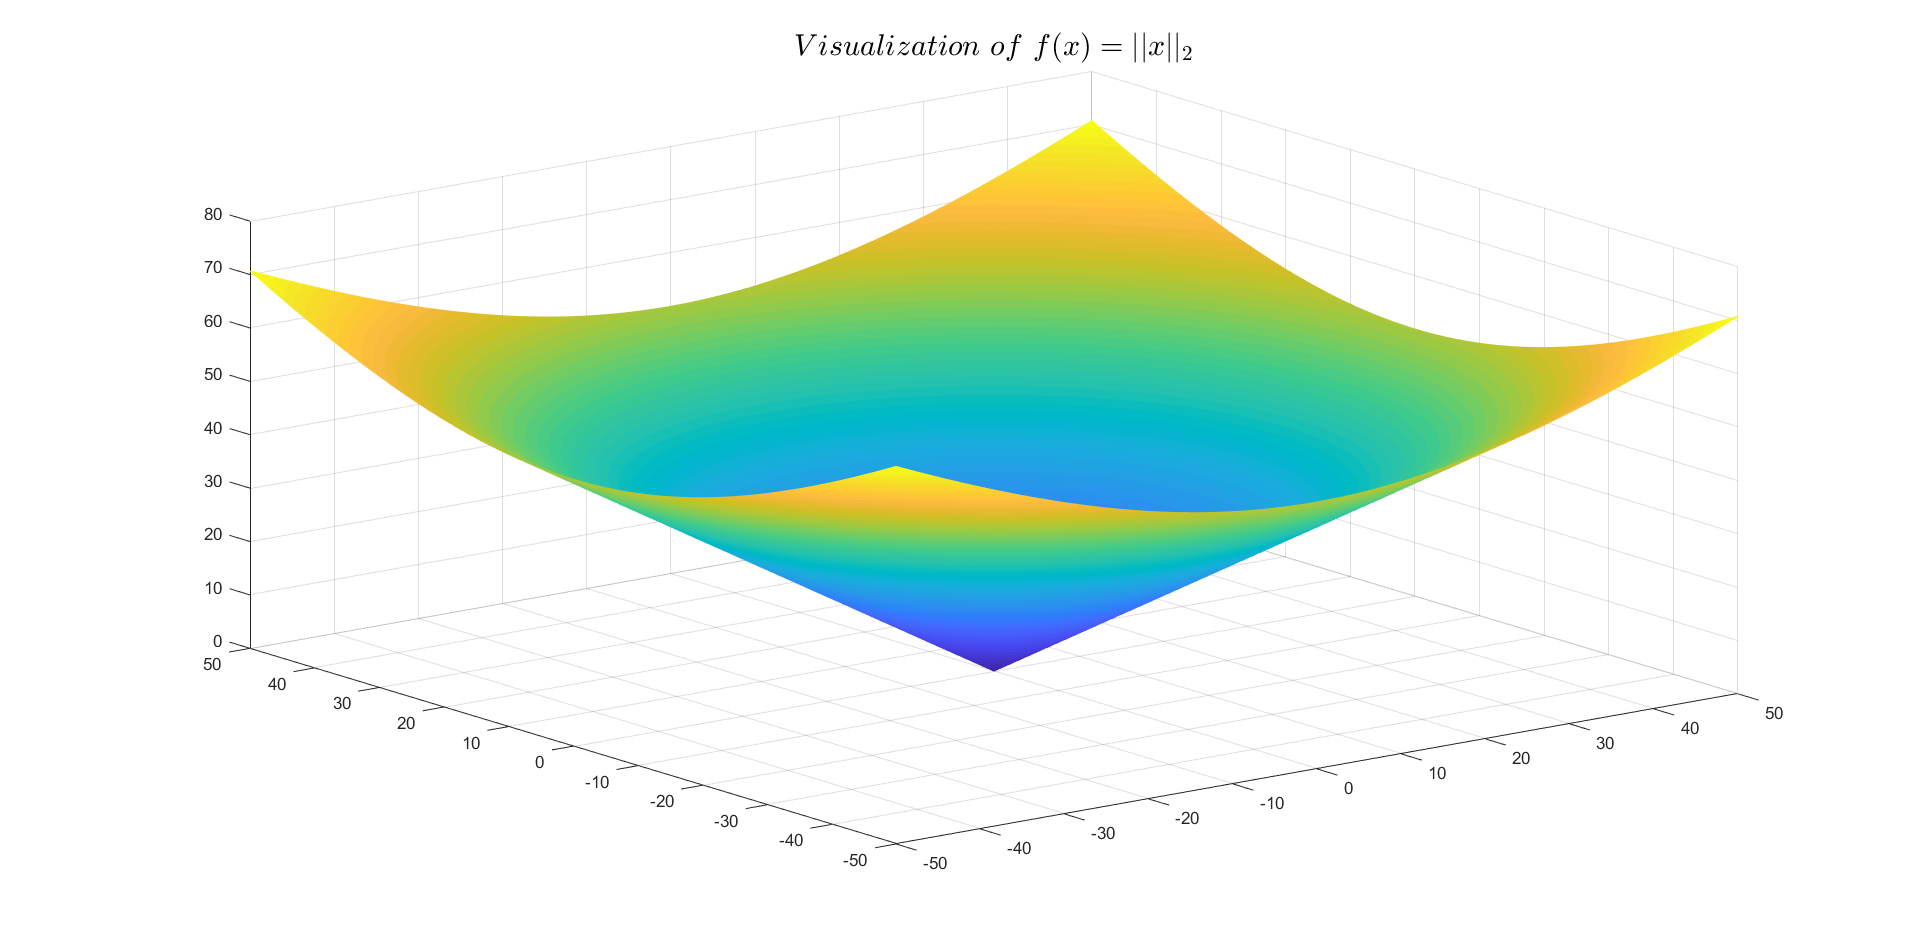
\includegraphics[width=\textwidth]{9.png}
	\caption{$f({\bf x})=||{\bf x}||_2$}
	\label{fig:9}
\end{figure}\\
\end{enumerate}
\newpage
\item
Let ${\bf A}\in\mathbb{R}^{m\times n}$, ${\bf b}\in\mathbb{R}^m$, and $f:\mathbb{R}^n\rightarrow \mathbb{R}$, with
$f({\bf x}) = \|{\bf Ax}-{\bf b}\|_2^2$. 
\begin{enumerate}
\item
Assuming that the columns of ${\bf A}$ are linearly independent and we will prove that $f$ is strictly convex.\\
f can be also be described as: 
\begin{equation}
	\begin{split}
		f({\bf x})&=\|{\bf Ax}-{\bf b}\|_2^2=({\bf A}{\bf x}-{\bf b})^T({\bf A}{\bf x}-{\bf b})\\
		&=({\bf x}^T{\bf A}^T-{\bf b}^T)({\bf A}{\bf x}-{\bf b})\\
		&={\bf x}^T{\bf A}^T{\bf A}{\bf x}-{\bf x}^T{\bf A}^T{\bf b}-{\bf b}^T{\bf A}{\bf x}+{\bf b}^T{\bf b}\\
		&\overset{*}{=}{\bf x}^T{\bf A}^T{\bf A}{\bf x}-{\bf b}^T{\bf A}{\bf x}-{\bf b}^T{\bf A}{\bf x}+{\bf b}^T{\bf b}\\
		&={\bf x}^T{\bf A}^T{\bf A}{\bf x}-2{\bf b}^T{\bf A}{\bf x}+{\bf b}^T{\bf b}
	\end{split}
\end{equation}
{(\bf *)} Since ${\bf x}^T{\bf A}^T{\bf b}$ is a scalar, then we can say that:\\
 ${\bf x}^T{\bf A}^T{\bf b}=({\bf x}^T{\bf A}^T{\bf b})^T=({\bf A}^T{\bf b})^T{\bf x}={\bf b}^T{\bf A}{\bf x}$\\
 
We can see that f is quadratic, therefore:
\begin{equation}
	\begin{split}
		\nabla f({\bf x}) &= 2{\bf A}^T{\bf A}{\bf x}-2{\bf b}^T{\bf A}\\
		\nabla^2(\bf x) & = 2{\bf A}^T{\bf A}
	\end{split}
\end{equation}

We will prove the first and second order derivatives.\\
\begin{itemize}
	\item
	For the first order derivative we need to calculate the partial derivatives of the terms ${\bf x}^T{\bf A}^T{\bf A}{\bf x}$, $2{\bf b}^T{\bf A}{\bf x}$ and ${\bf b}^T{\bf b}$.\\
	
	In order to prove the term ${\bf x}^T{\bf A}^T{\bf A}{\bf x}$, let ${\bf P}={\bf A}^T{\bf A}$. It is true that ${\bf x}^T{\bf P}{\bf x}=\sum_{i=1}^{n}x_i\big(\sum_{j=1}^{n}P_{ji}x_j\big)=$\\
	Therefore the partial derivatives:
	\begin{equation}
		\begin{split}
			\frac{(d{\bf x}^T{\bf P}{\bf x})}{dx_k}&=\frac{d}{dx_k}\sum_{i=1}^{n}x_i\big(\sum_{j=1}^{n} P_{ji}x_j\big)\\
			&=\frac{d}{dx_k}\sum_{i=1}^{n}\big(x_i^2P_{ii}+\sum_{j=1,j\ne i}^{n} x_iP_{ji}x_j\big)\\
			&=\frac{d}{dx_k}\sum_{i=1}^{n}\big(x_i^2P_{ii}\big)+\frac{d}{dx_k}\sum_{i=1}^{n}\big(\sum_{j=1,j\ne i}^{n} x_iP_{ji}x_j\big)\\
			&=2x_kP_{kk}+\sum_{i=1,i\ne k}^{n}P_{ik}x_i + \sum_{i=1,i\ne k}^{n}x_iP_{ki}\\
			&=2\sum_{i=1}^{n}P_{ki}x_i = 2{\bf P_k}^T{\bf x},\ where\ P_k\ the\ k-th\ column
		\end{split}
	\end{equation}
	After re-constructing the partial derivatives in a column vector we get $2{\bf P}{\bf x}=2{\bf A}^T{\bf A}{\bf x}$.\\
	
	For the calculation of the partial derivatives for the term $2{\bf b}^T{\bf A}{\bf x}$:\\
	Let ${\bf q}=2{\bf b}^T{\bf A}{\bf x}=2\sum_{i=1}^{n}\sum_{j=1}^{m}x_ib_jA{ji}$
	\begin{equation}
		\begin{split}
			\frac{(d{\bf b}^T{\bf A}{\bf x})}{dx_k}&=\frac{d}{dx_k}\big(2\sum_{i=1}^{n}\sum_{j=1}^{m}x_ib_jA{ji}\big)\\
			&=\sum_{j=1}^{m}b_jA{jk} = {\bf b}^T{\bf A_{k}},\ where\ A_k\ the\ k-th\ row
		\end{split}
	\end{equation}
	After re-constructing the partial derivatives in a column vector we get ${\bf b}^T{\bf A}$.\\
	
	The derivative of last term is obviously {\bf 0} because its independent of {\bf x}.\\
	
	Therefore $\nabla f({\bf x})= 2{\bf A}^T{\bf A}{\bf x}-2{\bf b}^T{\bf A}$.
	
	\item
	The second order differentiation of f.
	\begin{equation}
		\begin{split}
			\nabla^2 f({\bf x})_{ij}=\frac{d^2 f}{dx_id_xj}&=\frac{d}{x_j}\big( 2\sum_{k=1}^{n}P_{ik}x_k-\sum_{k=1}^{m}b_kA_{ki}\big) = 2P_{ij}
		\end{split}
	\end{equation}
	Therefore $\nabla^2 f({\bf x})=2{\bf P}=2{\bf A}^T{\bf A}$
\end{itemize}


In order to prove that f is strictly convex, it is  suffice to show that the hessian matrix is positive definite.\\
Firstly since the columns of {\bf A} are linearly independent then the equation ${\bf A}{\bf x}=0$ has only the trivial solution ${{\bf x}={\bf 0}}$.

By definition a matrix ${\bf M}$ is positive definite if and only the inequality ${\bf z}^T{\bf M}{\bf z}>0 \forall z\in \mathbb{R}^n-\{{\bf 0}\}$.\\
Replacing with the hessian:\\
\begin{equation}
	\begin{split}
		{\bf z}^T{\bf \nabla^2f({\bf x})}{\bf z}=2{\bf z}^T{\bf A}^T{\bf A}{\bf z}=2({\bf A}{\bf z})^T{\bf A}{\bf z} = 2||{\bf A}{\bf z}||^2\overset{*}{>} 0 \forall {\bf z}\in \mathbb{R}^n -\{{\bf 0}\}
	\end{split}
\end{equation}
{\bf (*)} The equality cannot be true because of the linear independency of {\bf A}.\\

Therefore ${\bf \nabla^2f({\bf x})}$ is positive definite and f is strictly convex.\\

\item Plots and contours of $f$ for $m=3$ and $n=2$. We generate a random ${\bf A}$ and ${\bf x_{seed}}$ using the function {\bf rand} of Matlab and we calculate ${\bf b}={\bf A}{\bf x_{seed}}$.\\
Also by generating a random error vector ${\bf e}$ using the function {\bf normrnd} with deviation 5 and median 3 we calculate ${\bf b_noise}={\bf A}{\bf x_{seed}}-{\bf e}$.\\
Using ${\bf A}$, ${\bf x_{seed}}$, ${\bf b}$ and ${\bf A}$, ${\bf x_{seed}}$, ${\bf b_{noise}}$ we calculate $f$ and $f_{noise}$ respectively.
\begin{figure}[h!]
	\centering
	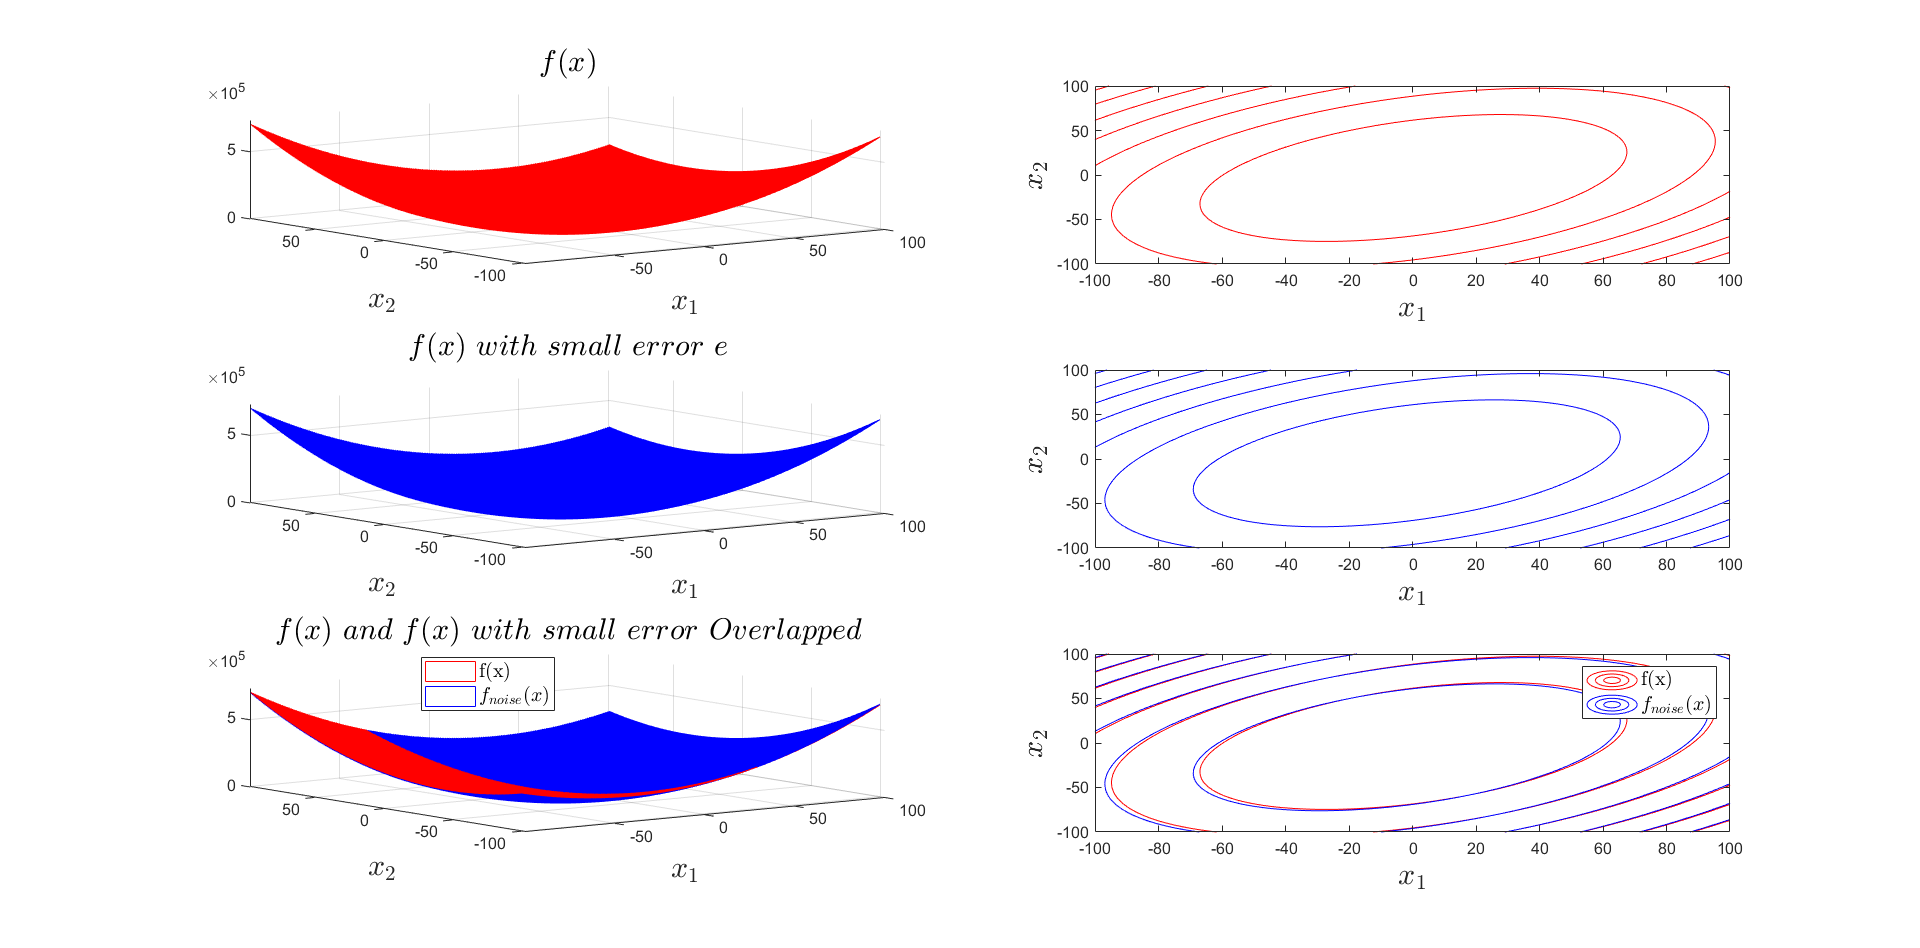
\includegraphics[width=\textwidth]{10.png}
	\caption{$f$ and $f_{noise}$ for $x_{seed}=(0.2853,-3.3435)^T$}
	\label{fig:10}
\end{figure}\\

From the graph and the contours of f observe that it is strictly convex as proved before.\\
Also adding the noise vector causes f to shift and change shape slightly but still remaining strictly convex. This explains the differences of f and the contour lines.

\end{enumerate}

\end{enumerate}
\newpage
The Matlab code used:
\lstset{style=myCustomMatlabStyle}
\lstinputlisting{Ex1.m}


\end{document}
